\documentclass[notitlepage]{revtex4-1}

\usepackage{graphicx}
\usepackage[margin=5pt]{subfig}
\usepackage[usenames]{color}
% \usepackage{xspace}
\definecolor{darkgreen}{rgb}{0.00,0.50,0.25}
\definecolor{darkblue}{rgb}{0.00,0.00,0.67}
\usepackage[breaklinks,pdftitle={ZeroDB whitepaper}, pdfauthor={Michael Egorov},colorlinks,urlcolor=blue,citecolor=darkgreen,linkcolor=darkblue]{hyperref}
\usepackage[usenames]{color}
\graphicspath{{pdf/}}

\begin{document}

\title{ZeroDB whitepaper}

\author{M. Egorov}
\email{michael@zerodb.io}
\author{M. Wilkison}
\email{maclane@zerodb.io}

\begin{abstract}
ZeroDB is an end-to-end encrypted database that enables clients to operate on (search, sort, query, and share) encrypted data without exposing encryption keys or cleartext data to the database server.
The familiar client-server architecture remains, but query logic and encryption keys are pushed client-side.
Since the server has no insight into the nature of the data, the risk of a server-side data breach is eliminated.
Even if adversaries successfully infiltrate the server, they will not have access to the cleartext data.

ZeroDB provides end-to-end encryption while maintaining much of the functionality expected of a modern database, such as full-text search, sort, and range queries.
Additionally, ZeroDB uses proxy re-encryption and/or delta key technology to enable secure, granular sharing of encrypted data without exposing keys to the server and without a risk of sharing the same encryption key between all users of the database.
\end{abstract}

\date{\today}
\maketitle

\section{Introduction}

Review of existing systems needed:~\cite{cipherbase}~\cite{cryptdb}~\cite{gentry}

\section{Query protocol}

Basis of the end-to-end encrypted query protocol is following.
The client interacts with the server during the execution of a query over a series of multiple round trips.
An encrypted index is stored on the server as a B-Tree, and the client traverses this index remotely to retrieve the necessary encrypted records.
Buckets which the index consists of are encrypted before being uploaded to the server and decrypted only on the side of the client.

\subsection{Keyword search}
\begin{figure}
	\begin{center}
        \subfloat{\label{fig:tree-traversal}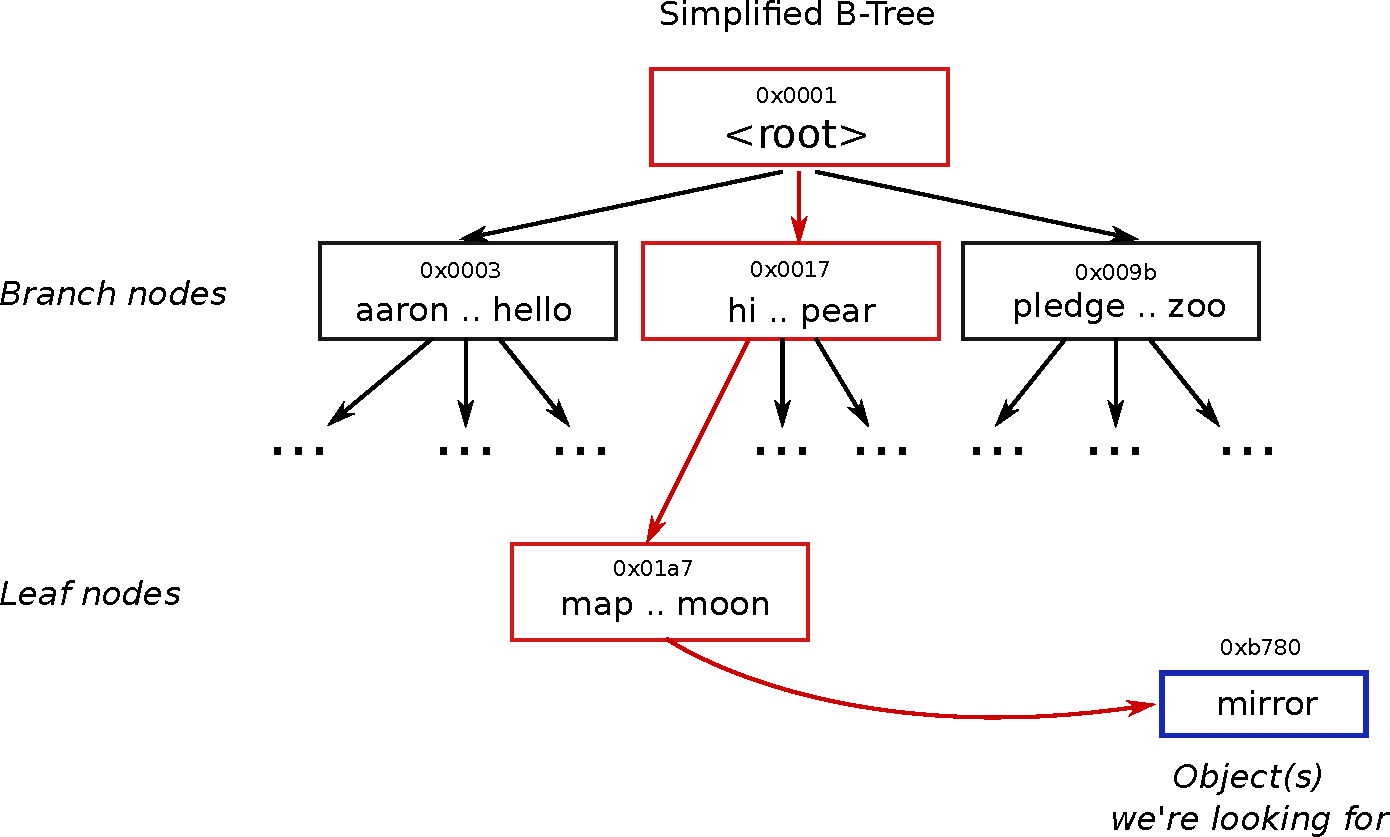
\includegraphics[width=0.47\columnwidth]{btree-traverse.pdf}}
        \qquad
		\subfloat{\label{fig:communication}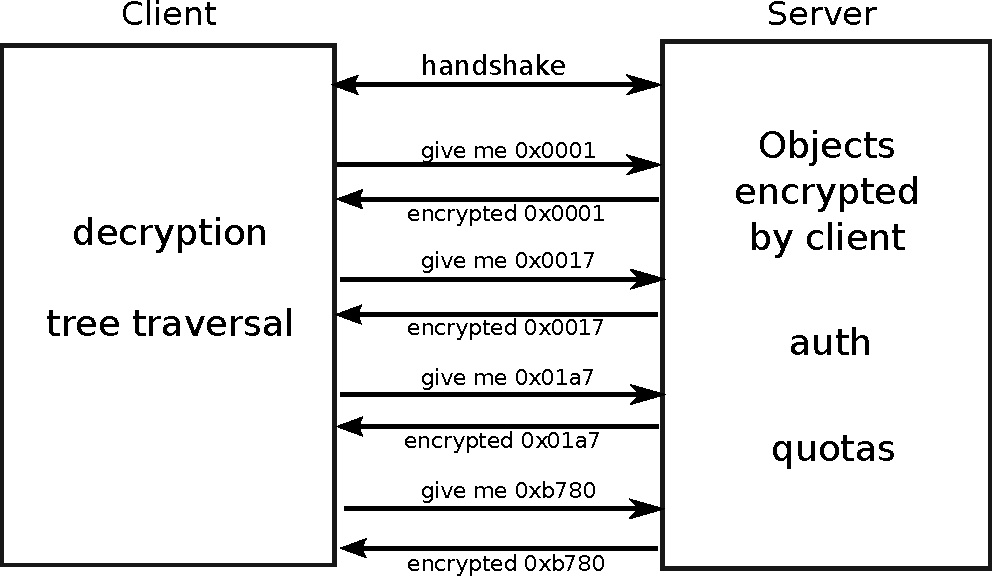
\includegraphics[width=0.47\columnwidth]{protocol.pdf}}
	\end{center}
	\caption[Calibration with the condensation temperature]{
		\subref{fig:tree-traversal} Tree traversal
		\subref{fig:communication} Example of network communication
	}
	\label{fig:btree-protocol}
\end{figure}

\subsection{Range queries}

\subsection{Complex queries (multi-keyword search, multiple conditions)}

\subsection{Joins}

\section{Sharing data}

\section{Security analysis}

\section{Performance}

\bibliography{zerodb}

\end{document}

